\begin{minipage}{0.55\textwidth}
\begin{align*}
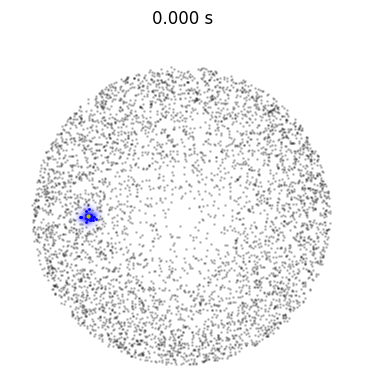
\includegraphics[width=0.49\textwidth]{simulation/3/frame_0.png}\hfill
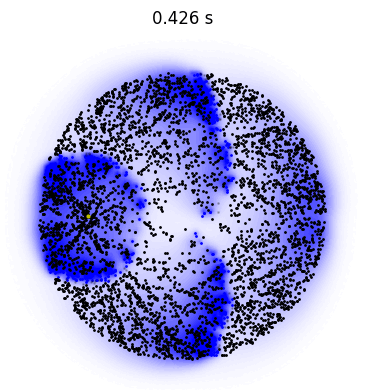
\includegraphics[width=0.49\textwidth]{simulation/3/frame_71.png}
\\[\smallskipamount]
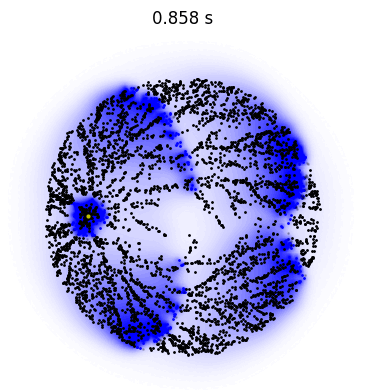
\includegraphics[width=0.49\textwidth]{simulation/3/frame_143.png}\hfill
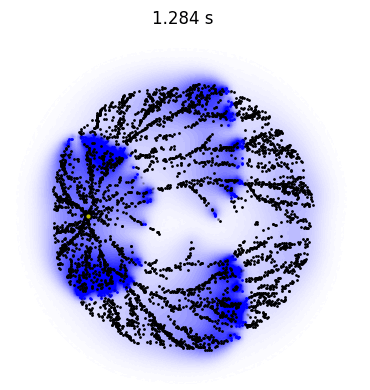
\includegraphics[width=0.49\textwidth]{simulation/3/frame_214.png}
\\[\smallskipamount]
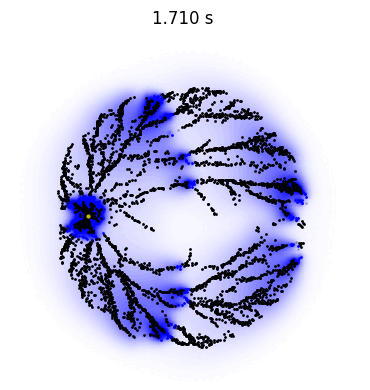
\includegraphics[width=0.49\textwidth]{simulation/3/frame_285.png}\hfill
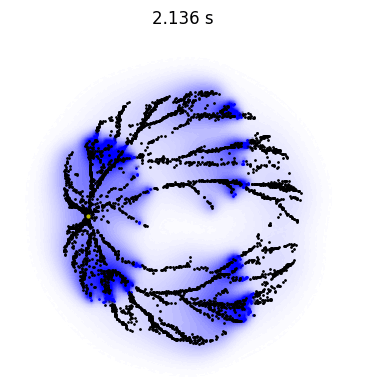
\includegraphics[width=0.49\textwidth]{simulation/3/frame_356.png}
\\[\smallskipamount]
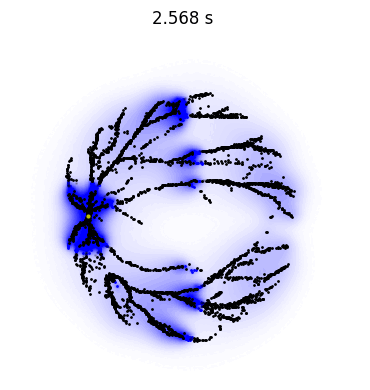
\includegraphics[width=0.49\textwidth]{simulation/3/frame_428.png}\hfill
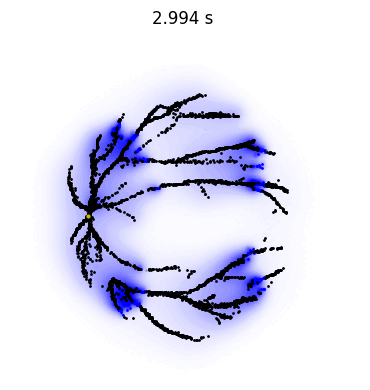
\includegraphics[width=0.49\textwidth]{simulation/3/frame_499.png}
\end{align*}
\end{minipage}
\begin{minipage}{0.45\textwidth}
\subsection{Low Density Center}
Contrary to the previous we used a disk with a lower density in the center in this simulation.
Again a pattern is clearly visible at about $1$s.
One can observe a very similar pattern to the Annulus simulation, a few branches going above the center and a few going below, but none going through.
The chemical diffusion clearly seems to prefer higher particle densities for its distribution.
Also similar to the annulus simulation we get a separation at the right.
\end{minipage}